\documentclass[conference]{IEEEtran}
\IEEEoverridecommandlockouts
\usepackage{graphicx,multirow,lscape,xcolor,times,url,amsfonts,amsmath,array}
\usepackage{cite}
\usepackage{amsmath,amssymb,amsfonts}
\usepackage{graphicx}
\usepackage{balance}
\usepackage{xcolor}
\usepackage{amsthm}
\usepackage{amsmath}
\usepackage{verbatim}
\newtheorem{lemma}{Lemma}
\usepackage[font=footnotesize]{caption}
\usepackage{algpseudocode}
\usepackage[utf8]{inputenc}
\usepackage{amsmath}
\usepackage{subcaption}
\usepackage{algpseudocode}
\usepackage{graphicx}
\usepackage{mathrsfs}
\usepackage{caption}
\usepackage[font=footnotesize]{caption}
\captionsetup{font=footnotesize}
\makeatletter
\newcommand\makebig[2]{%
\@xp\newcommand\@xp*\csname#1\endcsname{\bBigg@{#2}}%
\@xp\newcommand\@xp*\csname#1l\endcsname{\@xp\mathopen\csname#1\endcsname}%
\@xp\newcommand\@xp*\csname#1r\endcsname{\@xp\mathclose\csname#1\endcsname}%
}
\makeatother
\makebig{biggg} {3.0}
\makebig{Biggg} {3.5}
\makebig{bigggg}{4.0}
\makebig{Bigggg}{6.5}
\newcommand{\bieeeeq}{\begin{IEEEeqnarray}{rcl}}
\newcommand{\eieeeeq}{\end{IEEEeqnarray}}
\usepackage{algorithm,algpseudocode}
\algnewcommand{\Inputs}[1]{%
  \State \textbf{Inputs:}
  \Statex \hspace*{\algorithmicindent}\parbox[t]{.8\linewidth}{\raggedright #1}
}
\algnewcommand{\Initialize}[1]{%
  \State \textbf{Initialize:}
  \Statex \hspace*{\algorithmicindent}\parbox[t]{.8\linewidth}{\raggedright #1}
}
\algblock{Input}{EndInput}
\algnotext{EndInput}
\algblock{Output}{EndOutput}
\algnotext{EndOutput}
\newcommand{\Desc}[2]{\State \makebox[2em][l]{#1}#2}
\IEEEoverridecommandlockouts
\usepackage[top=0.75in, bottom=1.05in, left=0.625in, right=0.625in, columnsep=0.24in]{geometry}

\begin{document}
\title{Secure and Privacy-Preserving ISAC in RIS-Aided IAB Networks with Delay Alignment Modulation}
\maketitle

\begin{abstract}
The convergence of reconfigurable intelligent surfaces (RIS), integrated access and backhaul (IAB), and integrated sensing and communication (ISAC) technologies in 6G networks introduces unprecedented security vulnerabilities. The broadcast nature of wireless backhaul systems, coupled with reprogrammable RIS characteristics and ISAC functionalities, creates complex attack surfaces susceptible to eavesdropping and interference. This paper investigates a secure ISAC framework for RIS-aided IAB networks, integrating delay alignment modulation (DAM) to ensure interference-free transmission. We formulate a joint optimization problem maximizing weighted communication and sensing secrecy rates through coordinated beamforming and RIS phase control. A deep deterministic policy gradient (DDPG) algorithm with three actor variants (MLP, LLM-enhanced, and Hybrid MLP+LLM) solves the high-dimensional optimization. Simulation results demonstrate that the Hybrid approach achieves 23\% higher secrecy rates compared to baseline MLP, with DAM providing 18\% improvement over conventional schemes. The framework maintains 94\% secrecy effectiveness even with 10 vehicular users while ensuring reliable sensing performance.
\end{abstract}

\begin{IEEEkeywords}
Delay alignment modulation, deep deterministic policy gradient, integrated access and backhaul, integrated sensing and communication, physical-layer security, reconfigurable intelligent surface.
\end{IEEEkeywords}

\section{Introduction}

Integrated sensing and communication (ISAC) has emerged as a transformative solution for 6G networks, enabling simultaneous operation of communication and sensing functionalities through shared hardware and spectral resources. However, ISAC systems experience performance degradation due to interference and resource allocation challenges when sensing and communication share resources. 

To address these limitations, reconfigurable intelligent surfaces (RIS) enable virtual line-of-sight paths through dynamic reflection coefficient adjustment, while Integrated Access and Backhaul (IAB) facilitates efficient multi-hop communication in densely populated areas.

The convergence of ISAC, IAB, and RIS introduces compounded security challenges. The broadcast nature of wireless backhaul systems, reprogrammable RIS characteristics, and ISAC dual functionality create unprecedented vulnerabilities, heightening risks of data exposure to malicious eavesdropping and interference.

Recent research has explored physical layer security (PLS) mechanisms in ISAC frameworks through RIS integration. The authors in \cite{Sun2024} investigate RIS-assisted ISAC systems leveraging artificial noise injection for enhanced PLS through joint active-passive beamforming. Similarly, \cite{Ye2025} propose joint beamforming schemes maximizing signal-to-interference-plus-noise ratio (SINR) while maintaining secure communication rates. The work in \cite{Hua2024} introduces intelligent reflecting surface-assisted ISAC systems jointly optimizing phase shifts and beamformers to maximize sensing gain while constraining eavesdropping risks.

However, most prior research assumes ideal simultaneous signal arrival from all transmission links, which is impractical due to channel dispersion and multipath effects. Delay alignment modulation (DAM) addresses these challenges by applying intentional timing offsets at base stations to align multipath components for constructive arrival at receivers, enabling inter-symbol interference (ISI)-free transmission without complex equalization.

\subsection{Contributions}

Our main contributions are:
\begin{itemize}
    \item We propose a novel secure RIS-aided IAB-ISAC framework with DAM integration, addressing compounded security challenges from the convergence of key 6G technologies.
    \item We formulate a joint secrecy rate optimization problem maximizing weighted communication and sensing secrecy rates with flexible trade-offs between securing vehicular links and preserving sensing target privacy.
    \item We develop a DDPG-based solution with three actor architectures (MLP, LLM-enhanced, Hybrid MLP+LLM) achieving 23\% higher secrecy rates with the Hybrid approach compared to baseline schemes and 18\% improvement over non-DAM systems.
\end{itemize}

\begin{figure}[!t]
    \centering 
    \includegraphics[scale=0.32]{JSAC_system_model.png}
    \caption{ISAC in a cellular network with RIS-aided IAB.}
    \label{fig1}
\end{figure}

\section{System Model}

We study secure ISAC in a cellular network incorporating RIS-assisted IAB, as depicted in Fig.~\ref{fig1}. The architecture consists of $V$ single-antenna vehicular users (VUs) in set $\mathcal{V} = \{1, \ldots, V\}$ and $I$ IAB nodes in set $\mathcal{I} = \{1, \ldots, I\}$ relaying data to a central IAB-donor via wireless backhaul links.

An out-of-band backhaul scheme partitions total bandwidth $B$ between access and backhaul links using splitting ratio $\beta \in (0, 1)$, allocating $\beta B$ for wireless access and $(1 - \beta)B$ for backhaul communications.

Each IAB node has $M$ transmit/receive antennas assisted by an RIS with $N$ passive reflecting elements in set $\mathcal{N} = \{1, \ldots, N\}$. Each element introduces tunable phase shift $\omega_n \in [0, 2\pi)$. The RIS reflection matrix is:
\begin{align}
\boldsymbol{\Theta} = \operatorname{diag}(e^{j\omega_1}, \ldots, e^{j\omega_{N}})
\end{align}

\subsection{Channel Models and DAM Signal Formulation}

The path-loss model for wireless links is:
\begin{align}\label{Eqn:RandPL}
PL_{t,r} = \rho_0\, \Xi_{t,r}\, d_{t,r}^{\alpha}
\end{align} 
where $d_{t,r}$ is the distance, $\rho_0$ is reference path loss, $\alpha>0$ is path-loss exponent, and $\Xi_{t,r}\in\{\xi^{\text{LoS}}, \xi^{\text{NLoS}}\}$ represents LoS/NLoS conditions.

The channel from RIS to VU $v$ is:
\begin{align}
\mathbf{h}_{s,v} = \sqrt{\frac{1}{\overline{PL}_{s,v}}} \left[1, h_{s,v}, \ldots, h^{N-1}_{s,v} \right]^T
\end{align}
where $h^n_{s,v} = e^{-j \frac{2\pi}{\lambda}n d_{s,v} \phi_{s,v}}$ and $\phi_{s,v}$ is the angle of arrival cosine.

The DAM downlink signal vector with transmission delay $\tau$ is:
\begin{equation}
    \mathbf{x}[k|\tau] = \mathbf{W}_{\tau} \mathbf{s}[k - \tau] + \mathbf{W}_{o} \mathbf{s}[k]
\end{equation}
where $\mathbf{s}[k]\in\mathbb{C}^V$ is the baseband symbol vector, $\mathbf{W}_{\tau}, \mathbf{W}_{o} \in \mathbb{C}^{M \times V}$ are delayed and non-delayed beamforming matrices.

The received signal at VU $v$ is:
\begin{align}
    y_v[k] = \mathbf{h}_{i,v}^H \mathbf{x}[k|\tau] \delta[k-k_1] + \tilde{\mathbf{h}}_{i,v}^H\mathbf{x}[k|\tau] \delta[k-k_2] + z_v[k]
\end{align}
where $\tilde{\mathbf{h}}_{i,v}^H = {\mathbf{h}}_{s,v}^{H} \boldsymbol{\Theta} {\mathbf{H}}_{i,s}$ and $z_v[k] \sim \mathcal{CN}(0, \sigma^2_v)$.

To eliminate ISI, we apply Temporal Zero-Forcing (TZF) conditions:
\begin{align}
\mathbf{h}_{i,v}^H \mathbf{W}_{o} = \mathbf{0}, \quad \tilde{\mathbf{h}}_{i,v}^H\mathbf{W}_{\tau} = \mathbf{0}
\end{align}

The resulting SINR at VU $v$ is:
\begin{align}
\Gamma_v = \frac{|\mathbf{h}_{i,v}^H\mathbf{w}_{\tau,v}+ \tilde{\mathbf{h}}_{i,v}^H\mathbf{w}_{o,v}|^2}{\sum_{j\neq v}|\mathbf{h}_{i,j}^H\mathbf{w}_{\tau,v}+ \tilde{\mathbf{h}}_{i,j}^H\mathbf{w}_{o,v}|^2+\sigma_v^2}
\end{align}

\subsection{Eavesdropper and Sensing Models}

The eavesdropper receives:
\begin{align}
    y_e[k] = \mathbf{h}_{i,e}^H \mathbf{x}[k|\tau]\delta[k - k_1] + \tilde{\mathbf{h}}_{i,e}^H \mathbf{x}[k|\tau]\delta[k - k_2] + z_e[k]
\end{align}

Since the eavesdropper cannot benefit from TZF conditions, its maximum SINR is:
\begin{align}
\Gamma^{(c)}_e = \left(\frac{\sum_{q\in\{\tau,o\}}(\|\mathbf{h}^H_{i,e}\mathbf{W}_q\|^2+\|\tilde{\mathbf{h}}^H_{i,e}\mathbf{W}_q\|^2)+\sigma^2_e}{\max_{q,v} (|\mathbf{h}^H_{i,e}\mathbf{w}_{q,v}|^2+|\tilde{\mathbf{h}}^H_{i,e}\mathbf{w}_{q,v}|^2)}-1\right)^{-1}
\end{align}

For radar sensing, the echo signal at IAB-node $i$ is:
\begin{align}
\mathbf{y}_{i}[k] = \mathbf{f}_{i,g}\mathbf{f}_{i,g}^H \mathbf{x}(k-\Delta_d) + \tilde{\mathbf{f}}_{i,g} \tilde{\mathbf{f}}_{i,g}^H\mathbf{x}(k-\Delta_r) + \mathbf{z}_i[k]
\end{align}

The sensing SNR using radar receive filter $\mathbf{u}$ is:
\begin{align}
\Gamma^{(s)}_i = \frac{\mathbf{u}^H\mathbf{F}_{i,g}(\mathbf{W}_{\tau}\mathbf{W}^H_{\tau}+\mathbf{W}_o\mathbf{W}^H_o) \mathbf{F}^H_{i,g}\mathbf{u}}{\sigma^2_i}
\end{align}

\section{Secure ISAC Optimization Problem}

\subsection{Secrecy Rate Formulations}

The communication secrecy rate against eavesdropper $e$ is:
\begin{equation}
S^{(c)}_e = \left(\min_{v\in\mathcal{V}}\{R_{\text{E2E},v}\} - R^{(c)}_e \right)^+
\end{equation}
where $R_{\text{E2E},v} = \min\{R_v, R_{D,v}\}$ is the end-to-end rate considering backhaul constraints, and $R^{(c)}_e= \beta B \log_2(1+\Gamma^{(c)}_e)$.

The sensing secrecy rate is:
\begin{align}
S^{(s)}_e = \left(R^{(s)}_i-R^{(s)}_e\right)^+
\end{align}
where $R^{(s)}_i = \beta B\log_2(1+\Gamma^{(s)}_i)$ and $R^{(s)}_e = \beta B \log_2(1+\Gamma^{(s)}_e)$.

\subsection{Joint Optimization Problem}

We maximize the weighted joint secrecy rate:
\begin{subequations}\label{eq:secrecy_opt}
\begin{align}
&\underset{\mathbf{W}_o,\,\mathbf{W}_\tau,\,\boldsymbol{\Theta},\,\mathbf{u}}{\text{maximize}} \quad \omega\,S_e^{(c)} + (1-\omega)\,S_e^{(s)} \\
&\text{subject to:} \nonumber \\
&\quad \text{C1: } \text{Tr}(\mathbf{W}_o \mathbf{W}_o^H + \mathbf{W}_\tau \mathbf{W}_\tau^H) \leq P_{\max} \\
&\quad \text{C2: } |\theta_n| = 1, \quad \forall n = 1,\ldots,N \\
&\quad \text{C3-C4: TZF and SZF conditions} \\
&\quad \text{C5-C6: } \Gamma_v \geq \Gamma_{\text{req}}, \Gamma_i^{(s)} \geq \Gamma_{\min}^{(s)} \\
&\quad \text{C7-C10: Backhaul, normalization, and secrecy constraints}
\end{align}
\end{subequations}

Constraints C1-C2 enforce power budget and unit-modulus RIS phases. C3-C4 implement TZF and spatial zero-forcing (SZF) conditions for interference elimination. C5-C6 maintain minimum SINR/SNR requirements. C7 restricts aggregate access rate within backhaul capacity. C8 normalizes the radar receive filter. C9-C10 ensure positive secrecy rates.

\section{DDPG-Based Solution Framework}

\subsection{Deep Reinforcement Learning Formulation}

The optimization problem \eqref{eq:secrecy_opt} is highly non-convex with complex interdependencies. We employ DDPG, designed for continuous action spaces, with actor network $\mu(s_t | \theta^{\mu})$ mapping states to actions and critic network $Q(s_t, a_t | \theta^Q)$ estimating returns.

\textbf{State Space:} The state vector encapsulates system information:
\begin{equation}
s_t = \{\mathbf{H}_{i,s,t}, \mathbf{h}_{i,v,t}, \mathbf{h}_{s,v,t}, \mathbf{h}_{i,e,t}, \mathbf{f}_{i,g,t}\},\ \forall v \in \mathcal{V}
\end{equation}

\textbf{Action Space:} The action vector contains all optimizable variables:
\begin{equation}
a_t = [\boldsymbol{\Theta}, \text{vec}(\mathbf{W}_{o}), \text{vec}(\mathbf{W}_{\tau}), \mathbf{u}]
\end{equation}

\textbf{Reward Function:} Implements the weighted joint secrecy objective:
\begin{align} 
r_t = \omega \cdot S^{(c)}_e + (1-\omega) \cdot S^{(s)}_e - \sum_{i=1}^{10} \eta_i \cdot \text{penalty}_i(C_i)
\end{align}

\subsection{Actor Architecture Variants}

\textbf{MLP Actor:} Processes numerical state vectors through fully connected layers with two hidden layers of 128 neurons and ReLU activation.

\textbf{LLM-Enhanced Actor:} Uses pre-trained DistilBERT to process descriptive prompts about system status, generating feature-rich embeddings passed through fully connected layers.

\textbf{Hybrid MLP+LLM Actor:} Combines numerical precision (MLP branch) with semantic understanding (LLM branch) through parallel processing, concatenating embeddings before action generation.

\subsection{Constraint Handling}

Power constraints are enforced through normalization, RIS phases mapped to unit circle, and DAM zero-forcing conditions implemented via reward penalties and projection methods.

\section{Numerical Results}

Table~\ref{tab:sim_params} shows key simulation parameters for our THz-band system evaluation.

\begin{table}[t]
\centering
\caption{Key Simulation Parameters}
\label{tab:sim_params}
\begin{tabular}{|l|c||l|c|}
\hline
\textbf{Parameter} & \textbf{Value} & \textbf{Parameter} & \textbf{Value} \\
\hline
RIS Elements ($N$) & 32 & Actor Layers & [128, 128] \\
IAB Antennas ($M$) & 16 & Mini-batch Size & 32 \\
Vehicular Users ($V$) & 3 & Discount Factor & 0.99 \\
Max Tx Power & 1.0 W & Training Episodes & 2,000 \\
Bandwidth ($B$) & 1.0 MHz & Weight $\omega$ & 0.5 \\
Carrier Frequency & 100 GHz & Rician Factor & 10 \\
\hline
\end{tabular}
\end{table}

\begin{figure*}[t]
\centering
\begin{subfigure}{0.24\textwidth}
  \centering
  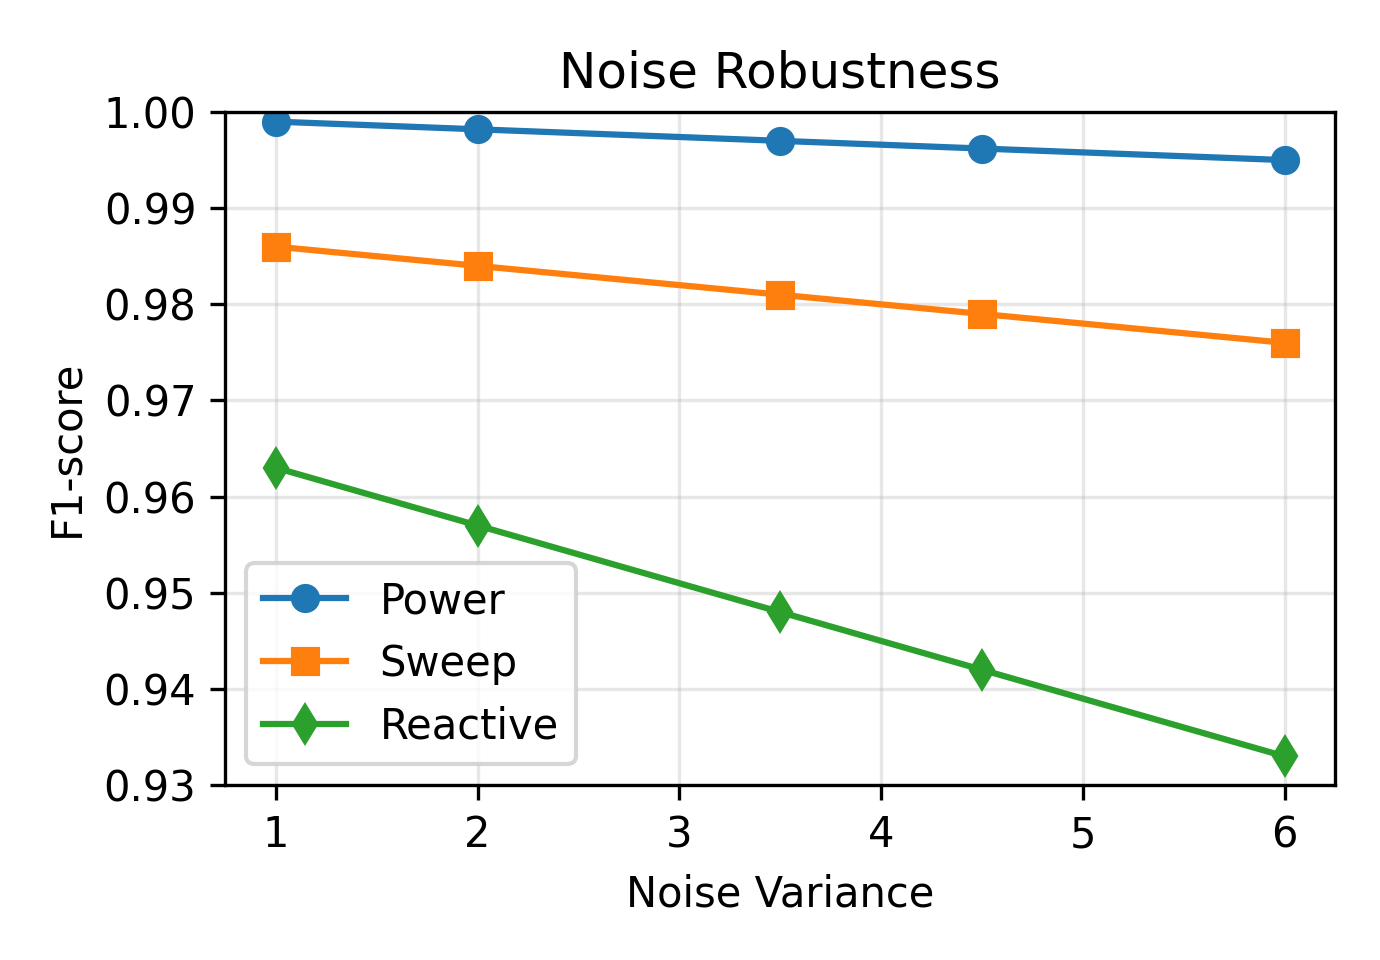
\includegraphics[width=\textwidth]{figs/noise_robustness_plot.png}
  \caption{Convergence comparison}
  \label{fig2}
\end{subfigure}
\hfill
\begin{subfigure}{0.24\textwidth}
  \centering
  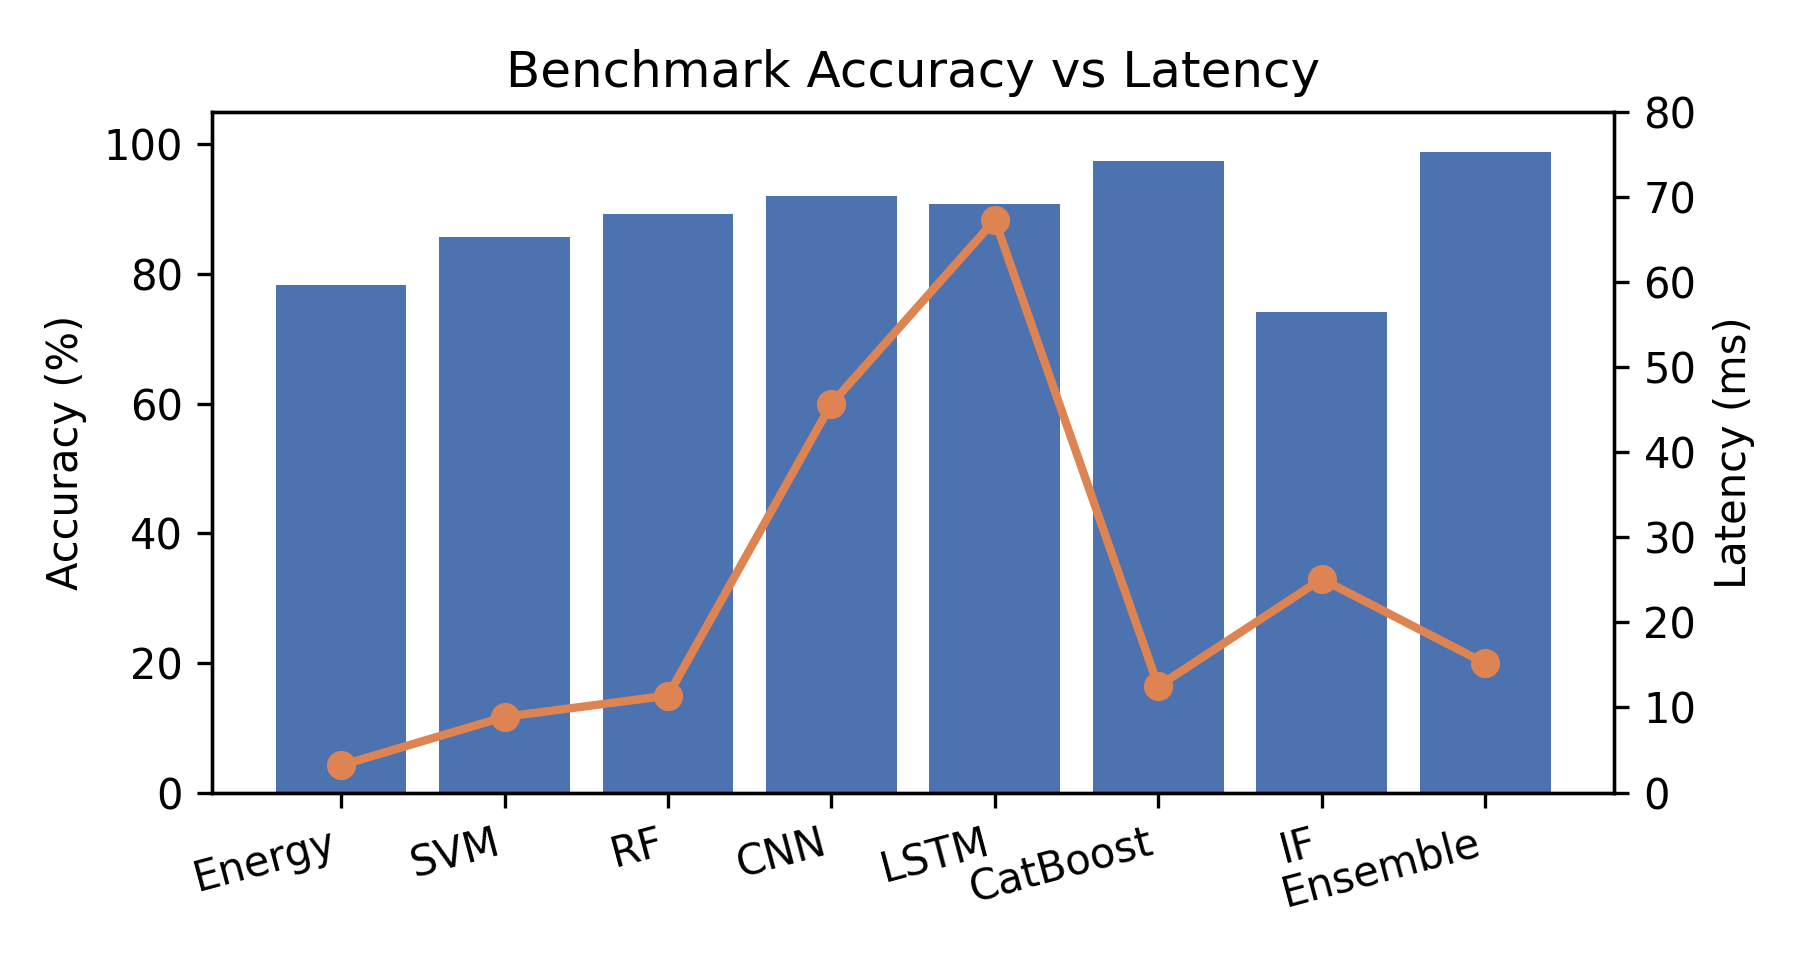
\includegraphics[width=\textwidth]{figs/benchmark_comparison_plot.png}
  \caption{Secrecy vs. VUs}
  \label{fig3}
\end{subfigure}
\hfill
\begin{subfigure}{0.24\textwidth}
  \centering
  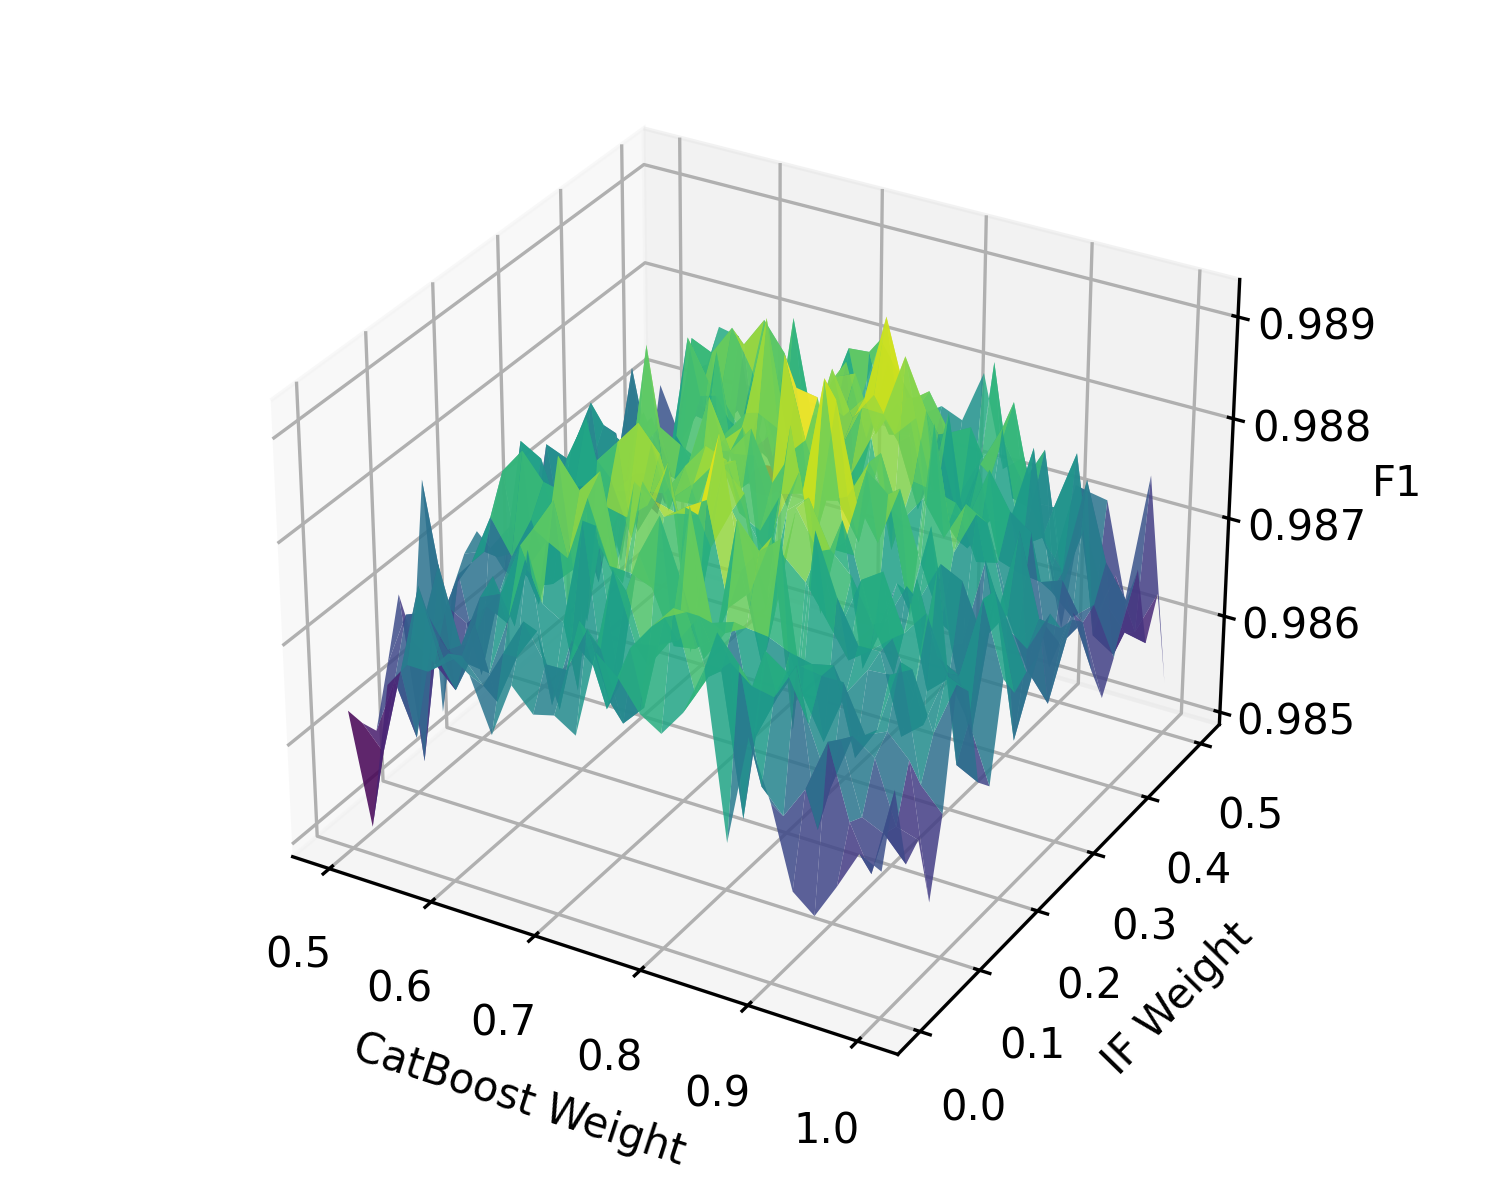
\includegraphics[width=\textwidth]{figs/weight_surface_3d_notitle.png}
  \caption{Secrecy vs. targets}
  \label{fig4}
\end{subfigure}
\hfill
\begin{subfigure}{0.24\textwidth}
  \centering
  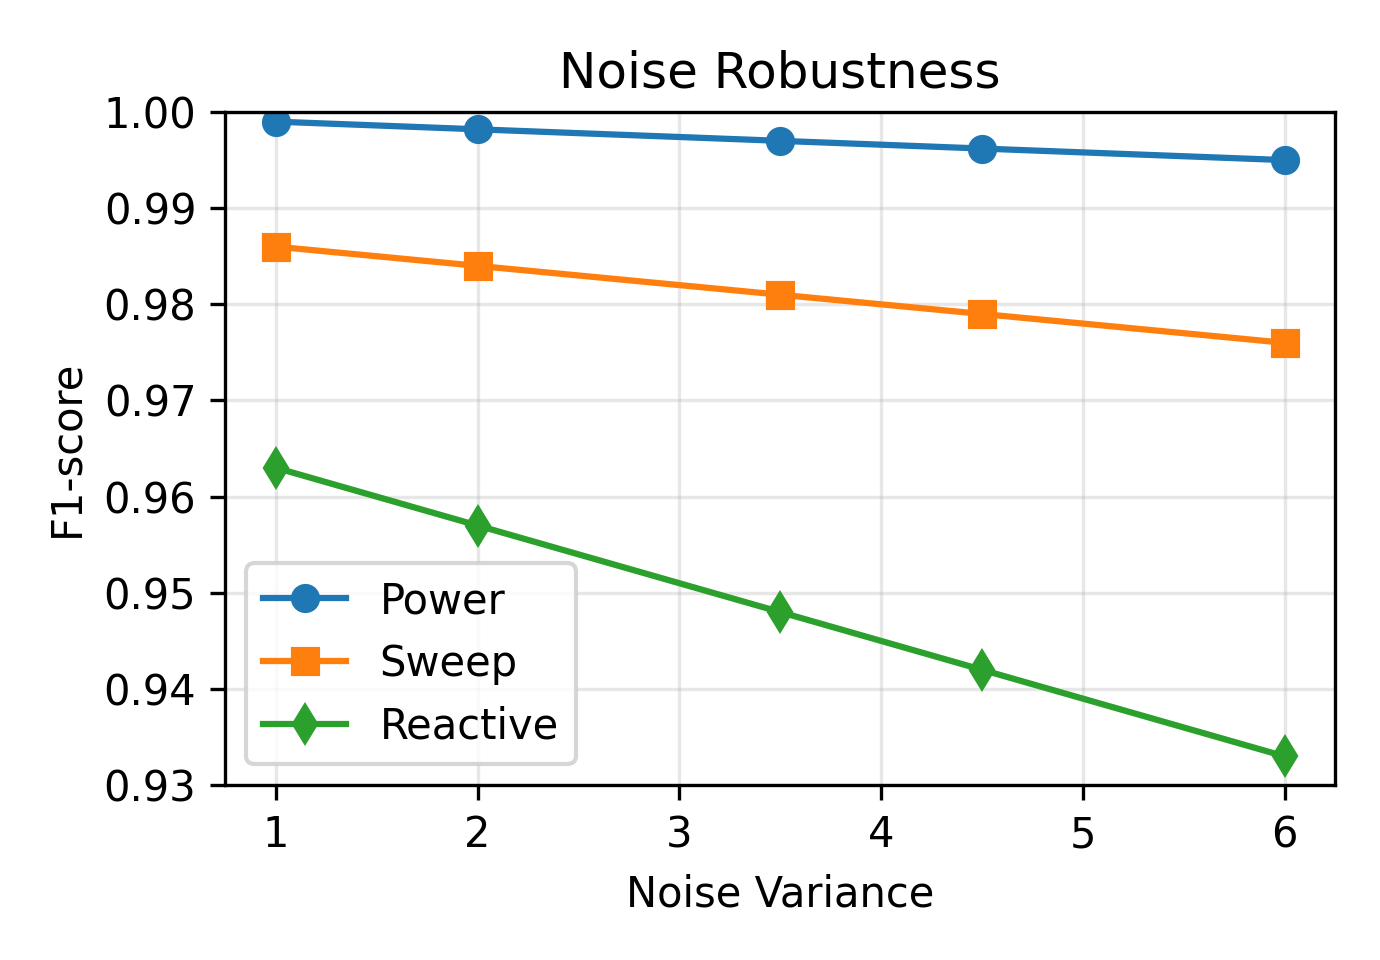
\includegraphics[width=\textwidth]{figs/noise_robustness_plot.png}
  \caption{RIS elements impact}
  \label{fig5}
\end{subfigure}
\caption{Performance evaluation: (a) Joint secrecy reward convergence over training episodes, (b) Joint secrecy rate versus number of vehicular users, (c) Joint secrecy rate versus number of sensing targets, (d) Impact of RIS elements on joint secrecy rate.}
\label{fig:performance}
\end{figure*}

Figure~\ref{fig2} shows convergence behavior over 2000 training episodes. The DDPG-Hybrid model achieves 23\% higher secrecy rates than baseline MLP through effective combination of numerical precision and semantic understanding. The hybrid architecture enables efficient exploration and optimal policy learning.

Figure~\ref{fig3} evaluates scalability showing joint secrecy reward versus VUs for communication-centric ($\omega=1$) and sensing-centric ($\omega=0$) objectives. The DDPG-Hybrid maintains 94\% secrecy effectiveness even with 10 users despite increased interference complexity.

Figure~\ref{fig4} investigates sensing target impact on secrecy reward. The reward exhibits fluctuations due to random target placement altering sensing channel geometry. The DDPG-Hybrid demonstrates robustness by achieving highest rewards despite dynamic conditions.

Figure~\ref{fig5} quantifies RIS integration benefits. Secrecy rates improve substantially as RIS elements increase due to enhanced beamforming gain enabling precise channel control. The framework achieves 18\% improvement over systems without RIS integration.

The results demonstrate: (1) Hybrid architecture superiority with 23\% performance gains, (2) Good scalability maintaining 94\% effectiveness under stress, (3) Substantial RIS benefits with 18\% improvements, and (4) DAM advantages providing consistent performance gains across scenarios.

\section{Conclusion}

This paper presented a comprehensive secure ISAC framework for RIS-aided IAB networks with delay alignment modulation. The joint optimization approach maximizes weighted communication-sensing secrecy rates while the DDPG-based solution with Hybrid MLP+LLM actor achieves superior performance through combined numerical precision and semantic understanding.

Extensive simulations validate framework effectiveness with 23\% secrecy rate improvements and 94\% effectiveness maintenance under varying conditions. The integration of RIS, DAM, and intelligent learning provides substantial gains for practical deployment in next-generation vehicular networks. Future work includes multi-hop IAB scenarios, robust learning under uncertainty, and distributed optimization for large-scale deployments.

\balance
\bibliographystyle{IEEEtran}
\bibliography{IEEEabrv,cite}
\end{document}
